In Section \ref{sec:dto_caching} the issue of
creating Data Transfer Objects with ClusterJ was introduced. In Figure
\ref{fig:impl_dto_no_cache} is depicted the time needed to create a number of
DTOs and persist them in the database. The evaluation of the Caching
mechanism was done both with a micro-benchmark but also with simulations
measuring the time to commit a Transaction State in the database,
the cluster utilization and also the number of heartbeats that the
scheduler is processing. The simulations were performed in the second
type of setup.

\begin{figure}
\centering
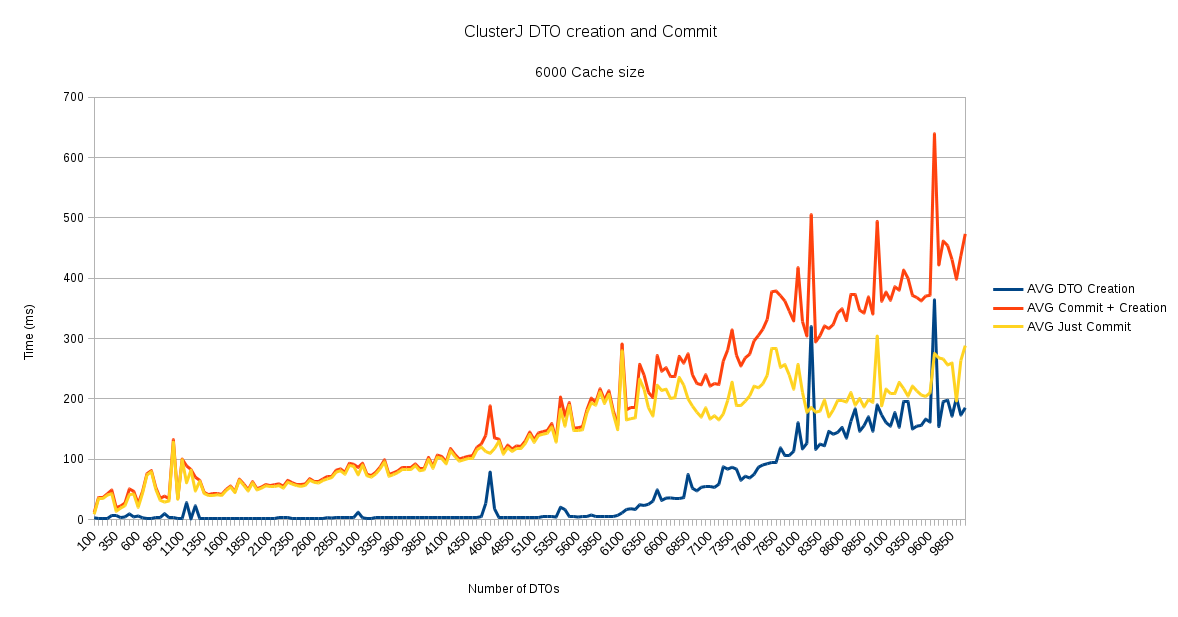
\includegraphics[scale=0.5]{resources/images/Evaluation/dto_creation_cache_bench.png}
\caption{DTO creation and commit with cache enabled}
\label{fig:ev_dto_creation_bench}
\end{figure}

In Figure \ref{fig:ev_dto_creation_bench} is the result of the same
micro-benchmark performed in Section \ref{sec:dto_caching} but with
the Caching mechanism. The blue line is the creation time of DTOs, the
yellow line is the actual commit time and the red one is both the
creation and the commit time. The cache size of the sessions was 6000
objects. The ``creation'' time in the second case is almost
zero and orders of magnitude less, until the cache limit is reached. Even when the number of DTOs
requested are more than the cache size, it is still much faster. At
the time the benchmark was done, the cache size of the sessions was
fixed to a number. It is expected the performance to be better with the
dynamic size of the cache.

The next evaluation parameter is the mean time for a Transaction State
to be committed in the database. The parameters of the cache are
outlined in Table \ref{tab:ev_cache_conf}. It is not possible to cache
all the DTO types mainly for two reasons. First, it would take more
time to fill-up the cache with more types which would result in
very few \emph{ready} sessions. So the transactions would use
non-cached sessions or even worse fall-back to creating new
sessions. The second reason is memory related. Even though DTOs are
not allocated on the heap of the JVM and do not account to Java
garbage collection, they still consume memory from the machine that
could be used for scheduling decisions or handling of heartbeats. In
Figure \ref{fig:ev_cache_ts_commit} is the average commit time of a
TransactionState object with cache-enabled and cache-disabled
sessions. Even with a cluster size of 2000 nodes there is a small
difference in the commit time. As the number of NodeManagers grows,
the difference is getting wider reaching almost 20 ms in 10000 nodes
cluster.

\begin{table}
\centering
\begin{tabular}{| c | c | c | c |}
\hline
\textbf{Type} & \textbf{Min. size} & \textbf{Max. size} & \textbf{Step}\\
\hline
\hline
PendingEventDTO & 12000 & 25000 & 400\\
\hline
NodeHBResponseDTO & 2000 & 10000 & 200\\
\hline
UpdatedContainerInfoDTO & 2000 & 10000 & 200\\
\hline
\end{tabular}
\caption{Cache mechanism configuration}
\label{tab:ev_cache_conf}
\end{table}

\begin{figure}
\centering
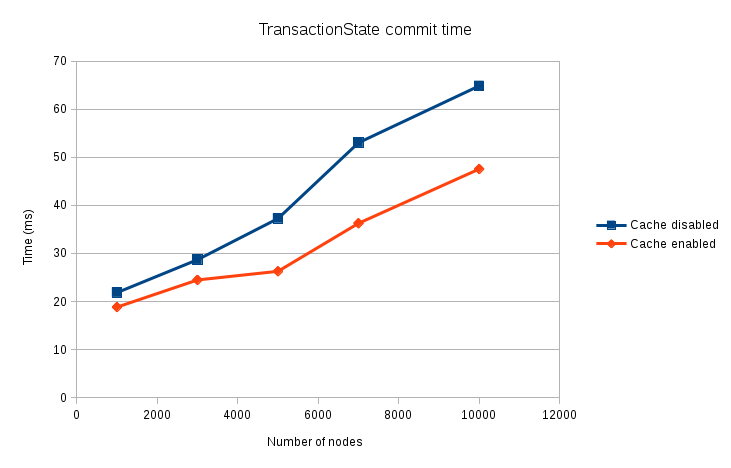
\includegraphics[scale=0.6]{resources/images/Evaluation/dto_cache_ts_commit.png}
\caption{TS commit time with and without cache}
\label{fig:ev_cache_ts_commit}
\end{figure}

\begin{figure}
\centering
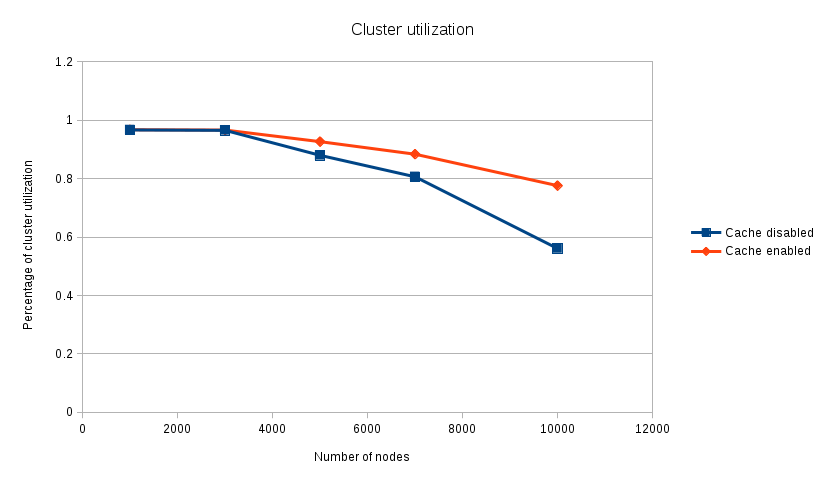
\includegraphics[scale=0.6]{resources/images/Evaluation/dto_cache_cluster_util.png}
\caption{Cluster utilization with and without cache}
\label{fig:ev_cache_cluster_util}
\end{figure}

The improvement in the commit time is reflected in the cluster
utilization as illustrated in Figure \ref{fig:ev_cache_cluster_util}.
Until 3000 nodes there is no difference in the utilization but the more
NodeManagers in the simulation, the bigger the difference is. In 10000
nodes simulation the cluster utilization increased from 56$\%$ to
77$\%$ and the launched containers from 167177 to 247032 (Figure
\ref{fig:ev_cache_containers}).

\begin{figure}
\centering
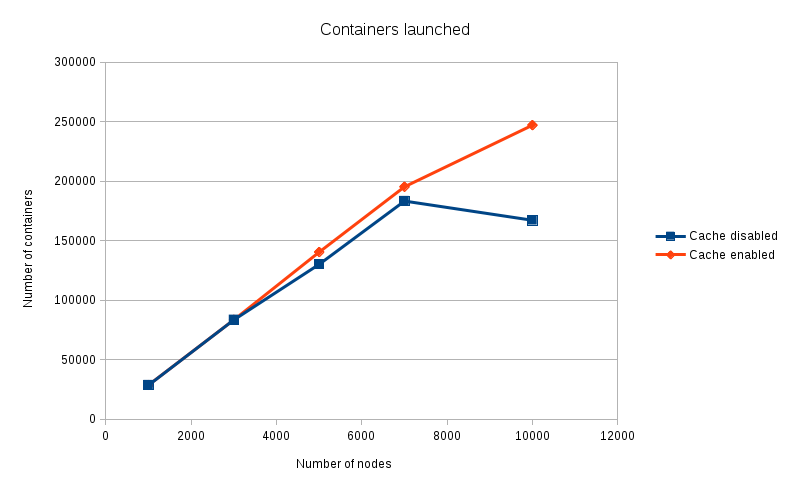
\includegraphics[scale=0.6]{resources/images/Evaluation/dto_cache_containers.png}
\caption{Containers launched with and without cache}
\label{fig:ev_cache_containers}
\end{figure}

\begin{figure}
\centering
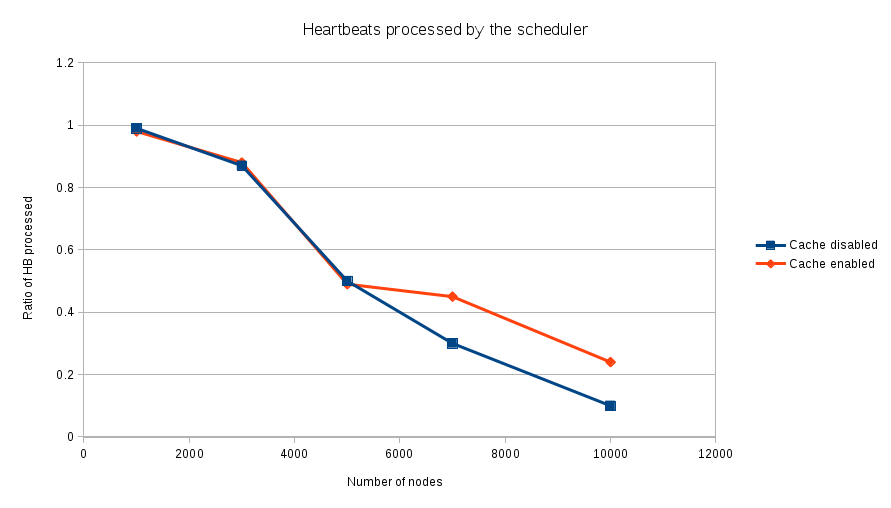
\includegraphics[scale=0.6]{resources/images/Evaluation/dto_cache_hb_processed.png}
\caption{HB processed with and without cache}
\label{fig:ev_cache_hb_processed}
\end{figure}

Finally, the number of heartbeats processed by the scheduler node has
also been increased but  still is quite low
affecting the scheduling decisions. In Figure
\ref{fig:ev_cache_hb_processed} is depicted the ratio of
heartbeats processed by the RM over the total number of
heartbeats. For a 10000 nodes cluster the ratio is still very low but
until 5000 NodeManagers is quite acceptable.